\documentclass[1p]{elsarticle_modified}
%\bibliographystyle{elsarticle-num}

%\usepackage[colorlinks]{hyperref}
%\usepackage{abbrmath_seonhwa} %\Abb, \Ascr, \Acal ,\Abf, \Afrak
\usepackage{amsfonts}
\usepackage{amssymb}
\usepackage{amsmath}
\usepackage{amsthm}
\usepackage{scalefnt}
\usepackage{amsbsy}
\usepackage{kotex}
\usepackage{caption}
\usepackage{subfig}
\usepackage{color}
\usepackage{graphicx}
\usepackage{xcolor} %% white, black, red, green, blue, cyan, magenta, yellow
\usepackage{float}
\usepackage{setspace}
\usepackage{hyperref}

\usepackage{tikz}
\usetikzlibrary{arrows}

\usepackage{multirow}
\usepackage{array} % fixed length table
\usepackage{hhline}

%%%%%%%%%%%%%%%%%%%%%
\makeatletter
\renewcommand*\env@matrix[1][\arraystretch]{%
	\edef\arraystretch{#1}%
	\hskip -\arraycolsep
	\let\@ifnextchar\new@ifnextchar
	\array{*\c@MaxMatrixCols c}}
\makeatother %https://tex.stackexchange.com/questions/14071/how-can-i-increase-the-line-spacing-in-a-matrix
%%%%%%%%%%%%%%%

\usepackage[normalem]{ulem}

\newcommand{\msout}[1]{\ifmmode\text{\sout{\ensuremath{#1}}}\else\sout{#1}\fi}
%SOURCE: \msout is \stkout macro in https://tex.stackexchange.com/questions/20609/strikeout-in-math-mode

\newcommand{\cancel}[1]{
	\ifmmode
	{\color{red}\msout{#1}}
	\else
	{\color{red}\sout{#1}}
	\fi
}

\newcommand{\add}[1]{
	{\color{blue}\uwave{#1}}
}

\newcommand{\replace}[2]{
	\ifmmode
	{\color{red}\msout{#1}}{\color{blue}\uwave{#2}}
	\else
	{\color{red}\sout{#1}}{\color{blue}\uwave{#2}}
	\fi
}

\newcommand{\Sol}{\mathcal{S}} %segment
\newcommand{\D}{D} %diagram
\newcommand{\A}{\mathcal{A}} %arc


%%%%%%%%%%%%%%%%%%%%%%%%%%%%%5 test

\def\sl{\operatorname{\textup{SL}}(2,\Cbb)}
\def\psl{\operatorname{\textup{PSL}}(2,\Cbb)}
\def\quan{\mkern 1mu \triangleright \mkern 1mu}

\theoremstyle{definition}
\newtheorem{thm}{Theorem}[section]
\newtheorem{prop}[thm]{Proposition}
\newtheorem{lem}[thm]{Lemma}
\newtheorem{ques}[thm]{Question}
\newtheorem{cor}[thm]{Corollary}
\newtheorem{defn}[thm]{Definition}
\newtheorem{exam}[thm]{Example}
\newtheorem{rmk}[thm]{Remark}
\newtheorem{alg}[thm]{Algorithm}

\newcommand{\I}{\sqrt{-1}}
\begin{document}

%\begin{frontmatter}
%
%\title{Boundary parabolic representations of knots up to 8 crossings}
%
%%% Group authors per affiliation:
%\author{Yunhi Cho} 
%\address{Department of Mathematics, University of Seoul, Seoul, Korea}
%\ead{yhcho@uos.ac.kr}
%
%
%\author{Seonhwa Kim} %\fnref{s_kim}}
%\address{Center for Geometry and Physics, Institute for Basic Science, Pohang, 37673, Korea}
%\ead{ryeona17@ibs.re.kr}
%
%\author{Hyuk Kim}
%\address{Department of Mathematical Sciences, Seoul National University, Seoul 08826, Korea}
%\ead{hyukkim@snu.ac.kr}
%
%\author{Seokbeom Yoon}
%\address{Department of Mathematical Sciences, Seoul National University, Seoul, 08826,  Korea}
%\ead{sbyoon15@snu.ac.kr}
%
%\begin{abstract}
%We find all boundary parabolic representation of knots up to 8 crossings.
%
%\end{abstract}
%\begin{keyword}
%    \MSC[2010] 57M25 
%\end{keyword}
%
%\end{frontmatter}

%\linenumbers
%\tableofcontents
%
\newcommand\colored[1]{\textcolor{white}{\rule[-0.35ex]{0.8em}{1.4ex}}\kern-0.8em\color{red} #1}%
%\newcommand\colored[1]{\textcolor{white}{ #1}\kern-2.17ex	\textcolor{white}{ #1}\kern-1.81ex	\textcolor{white}{ #1}\kern-2.15ex\color{red}#1	}

{\Large $\underline{12n_{0861}~(K12n_{0861})}$}

\setlength{\tabcolsep}{10pt}
\renewcommand{\arraystretch}{1.6}
\vspace{1cm}\begin{tabular}{m{100pt}>{\centering\arraybackslash}m{274pt}}
\multirow{5}{120pt}{
	\centering
	\includegraphics[width=112pt]{../../../GIT/diagram.site/Diagrams/png/2950_12n_0861.png}\\
\ \ \ A knot diagram\footnotemark}&
\allowdisplaybreaks
\textbf{Linearized knot diagam} \\
\cline{2-2}
 &
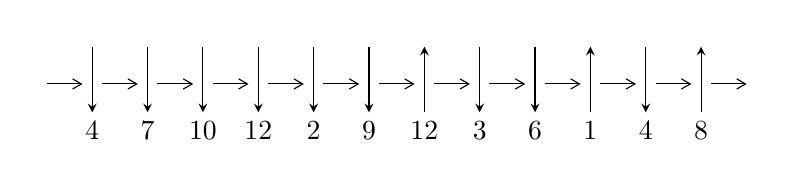
\begin{tikzpicture}[x=20pt, y=17pt]
	% nodes
	\node (C0) at (0, 0) {};
	\node (C1) at (1, 0) {};
	\node (C1U) at (1, +1) {};
	\node (C1D) at (1, -1) {4};

	\node (C2) at (2, 0) {};
	\node (C2U) at (2, +1) {};
	\node (C2D) at (2, -1) {7};

	\node (C3) at (3, 0) {};
	\node (C3U) at (3, +1) {};
	\node (C3D) at (3, -1) {10};

	\node (C4) at (4, 0) {};
	\node (C4U) at (4, +1) {};
	\node (C4D) at (4, -1) {12};

	\node (C5) at (5, 0) {};
	\node (C5U) at (5, +1) {};
	\node (C5D) at (5, -1) {2};

	\node (C6) at (6, 0) {};
	\node (C6U) at (6, +1) {};
	\node (C6D) at (6, -1) {9};

	\node (C7) at (7, 0) {};
	\node (C7U) at (7, +1) {};
	\node (C7D) at (7, -1) {12};

	\node (C8) at (8, 0) {};
	\node (C8U) at (8, +1) {};
	\node (C8D) at (8, -1) {3};

	\node (C9) at (9, 0) {};
	\node (C9U) at (9, +1) {};
	\node (C9D) at (9, -1) {6};

	\node (C10) at (10, 0) {};
	\node (C10U) at (10, +1) {};
	\node (C10D) at (10, -1) {1};

	\node (C11) at (11, 0) {};
	\node (C11U) at (11, +1) {};
	\node (C11D) at (11, -1) {4};

	\node (C12) at (12, 0) {};
	\node (C12U) at (12, +1) {};
	\node (C12D) at (12, -1) {8};
	\node (C13) at (13, 0) {};

	% arrows
	\draw[->,>={angle 60}]
	(C0) edge (C1) (C1) edge (C2) (C2) edge (C3) (C3) edge (C4) (C4) edge (C5) (C5) edge (C6) (C6) edge (C7) (C7) edge (C8) (C8) edge (C9) (C9) edge (C10) (C10) edge (C11) (C11) edge (C12) (C12) edge (C13) ;	\draw[->,>=stealth]
	(C1U) edge (C1D) (C2U) edge (C2D) (C3U) edge (C3D) (C4U) edge (C4D) (C5U) edge (C5D) (C6U) edge (C6D) (C7D) edge (C7U) (C8U) edge (C8D) (C9U) edge (C9D) (C10D) edge (C10U) (C11U) edge (C11D) (C12D) edge (C12U) ;
	\end{tikzpicture} \\
\hhline{~~} \\& 
\textbf{Solving Sequence} \\ \cline{2-2} 
 &
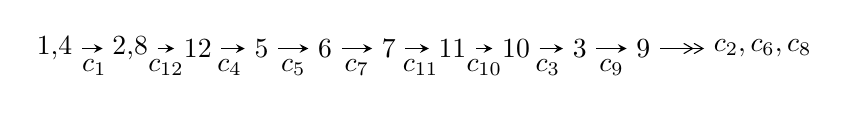
\begin{tikzpicture}[x=23pt, y=7pt]
	% node
	\node (A0) at (-1/8, 0) {1,4};
	\node (A1) at (17/16, 0) {2,8};
	\node (A2) at (17/8, 0) {12};
	\node (A3) at (25/8, 0) {5};
	\node (A4) at (33/8, 0) {6};
	\node (A5) at (41/8, 0) {7};
	\node (A6) at (49/8, 0) {11};
	\node (A7) at (57/8, 0) {10};
	\node (A8) at (65/8, 0) {3};
	\node (A9) at (73/8, 0) {9};
	\node (C1) at (1/2, -1) {$c_{1}$};
	\node (C2) at (13/8, -1) {$c_{12}$};
	\node (C3) at (21/8, -1) {$c_{4}$};
	\node (C4) at (29/8, -1) {$c_{5}$};
	\node (C5) at (37/8, -1) {$c_{7}$};
	\node (C6) at (45/8, -1) {$c_{11}$};
	\node (C7) at (53/8, -1) {$c_{10}$};
	\node (C8) at (61/8, -1) {$c_{3}$};
	\node (C9) at (69/8, -1) {$c_{9}$};
	\node (A10) at (11, 0) {$c_{2},c_{6},c_{8}$};

	% edge
	\draw[->,>=stealth]	
	(A0) edge (A1) (A1) edge (A2) (A2) edge (A3) (A3) edge (A4) (A4) edge (A5) (A5) edge (A6) (A6) edge (A7) (A7) edge (A8) (A8) edge (A9) ;
	\draw[->>,>={angle 60}]	
	(A9) edge (A10);
\end{tikzpicture} \\ 

\end{tabular} \\

\footnotetext{
The image of knot diagram is generated by the software ``\textbf{Draw programme}" developed by Andrew Bartholomew(\url{http://www.layer8.co.uk/maths/draw/index.htm\#Running-draw}), where we modified some parts for our purpose(\url{https://github.com/CATsTAILs/LinksPainter}).
}\phantom \\ \newline 
\centering \textbf{Ideals for irreducible components\footnotemark of $X_{\text{par}}$} 
 
\begin{align*}
I^u_{1}&=\langle 
-3.52500\times10^{352} u^{75}+2.44054\times10^{352} u^{74}+\cdots+7.62932\times10^{355} b-3.61083\times10^{356},\\
\phantom{I^u_{1}}&\phantom{= \langle  }1.06932\times10^{357} u^{75}-9.06361\times10^{356} u^{74}+\cdots+1.73575\times10^{360} a+3.60585\times10^{361},\\
\phantom{I^u_{1}}&\phantom{= \langle  }u^{76}- u^{75}+\cdots+300923 u-22751\rangle \\
I^u_{2}&=\langle 
1.63851\times10^{16} u^{28}-1.05439\times10^{17} u^{27}+\cdots+2.06022\times10^{16} b+2.70631\times10^{16},\\
\phantom{I^u_{2}}&\phantom{= \langle  }-1.08672\times10^{17} u^{28}+6.98492\times10^{17} u^{27}+\cdots+2.06022\times10^{16} a-1.87524\times10^{17},\;u^{29}-6 u^{28}+\cdots+3 u+1\rangle \\
\\
\end{align*}
\raggedright * 2 irreducible components of $\dim_{\mathbb{C}}=0$, with total 105 representations.\\
\footnotetext{All coefficients of polynomials are rational numbers. But the coefficients are sometimes approximated in decimal forms when there is not enough margin.}
\newpage
\renewcommand{\arraystretch}{1}
\centering \section*{I. $I^u_{1}= \langle -3.52\times10^{352} u^{75}+2.44\times10^{352} u^{74}+\cdots+7.63\times10^{355} b-3.61\times10^{356},\;1.07\times10^{357} u^{75}-9.06\times10^{356} u^{74}+\cdots+1.74\times10^{360} a+3.61\times10^{361},\;u^{76}- u^{75}+\cdots+300923 u-22751 \rangle$}
\flushleft \textbf{(i) Arc colorings}\\
\begin{tabular}{m{7pt} m{180pt} m{7pt} m{180pt} }
\flushright $a_{1}=$&$\begin{pmatrix}1\\0\end{pmatrix}$ \\
\flushright $a_{4}=$&$\begin{pmatrix}0\\u\end{pmatrix}$ \\
\flushright $a_{2}=$&$\begin{pmatrix}1\\u^2\end{pmatrix}$ \\
\flushright $a_{8}=$&$\begin{pmatrix}-0.000616058 u^{75}+0.000522174 u^{74}+\cdots+215.201 u-20.7741\\0.000462033 u^{75}-0.000319890 u^{74}+\cdots-58.5348 u+4.73283\end{pmatrix}$ \\
\flushright $a_{12}=$&$\begin{pmatrix}-0.000551004 u^{75}+0.000291524 u^{74}+\cdots+274.093 u-26.3938\\0.000186949 u^{75}-0.000146137 u^{74}+\cdots-131.746 u+12.9652\end{pmatrix}$ \\
\flushright $a_{5}=$&$\begin{pmatrix}0.0000761766 u^{75}-0.000159869 u^{74}+\cdots-182.673 u+18.3344\\0.000150608 u^{75}-0.000110104 u^{74}+\cdots-11.9614 u+0.330376\end{pmatrix}$ \\
\flushright $a_{6}=$&$\begin{pmatrix}-0.0000399552 u^{75}+0.0000247574 u^{74}+\cdots-143.793 u+16.0999\\0.000269364 u^{75}-0.000203992 u^{74}+\cdots-35.2152 u+1.88871\end{pmatrix}$ \\
\flushright $a_{7}=$&$\begin{pmatrix}-0.000554392 u^{75}+0.000760906 u^{74}+\cdots+286.400 u-25.1589\\0.000189206 u^{75}-0.000484611 u^{74}+\cdots-184.889 u+14.2787\end{pmatrix}$ \\
\flushright $a_{11}=$&$\begin{pmatrix}-0.000551004 u^{75}+0.000291524 u^{74}+\cdots+274.093 u-26.3938\\0.000221974 u^{75}-0.000216748 u^{74}+\cdots-197.293 u+18.8687\end{pmatrix}$ \\
\flushright $a_{10}=$&$\begin{pmatrix}-0.000772978 u^{75}+0.000508271 u^{74}+\cdots+471.387 u-45.2625\\0.000221974 u^{75}-0.000216748 u^{74}+\cdots-197.293 u+18.8687\end{pmatrix}$ \\
\flushright $a_{3}=$&$\begin{pmatrix}-3.12392\times10^{-6} u^{75}-0.000182643 u^{74}+\cdots+63.4430 u-9.84321\\0.0000430791 u^{75}+0.000157885 u^{74}+\cdots+80.3500 u-6.25668\end{pmatrix}$ \\
\flushright $a_{9}=$&$\begin{pmatrix}-0.000272927 u^{75}-0.0000644983 u^{74}+\cdots+230.916 u-26.2228\\-0.0000751541 u^{75}+0.000223603 u^{74}+\cdots-12.0363 u+4.65606\end{pmatrix}$\\&\end{tabular}
\flushleft \textbf{(ii) Obstruction class $= -1$}\\~\\
\flushleft \textbf{(iii) Cusp Shapes $= -0.00205545 u^{75}+0.000950151 u^{74}+\cdots+1477.37 u-145.995$}\\~\\
\newpage\renewcommand{\arraystretch}{1}
\flushleft \textbf{(iv) u-Polynomials at the component}\newline \\
\begin{tabular}{m{50pt}|m{274pt}}
Crossings & \hspace{64pt}u-Polynomials at each crossing \\
\hline $$\begin{aligned}c_{1}\end{aligned}$$&$\begin{aligned}
&u^{76}+u^{75}+\cdots-300923 u-22751
\end{aligned}$\\
\hline $$\begin{aligned}c_{2}\end{aligned}$$&$\begin{aligned}
&u^{76}-2 u^{75}+\cdots-180357 u-34261
\end{aligned}$\\
\hline $$\begin{aligned}c_{3}\end{aligned}$$&$\begin{aligned}
&u^{76}-3 u^{75}+\cdots+950 u-239
\end{aligned}$\\
\hline $$\begin{aligned}c_{4},c_{11}\end{aligned}$$&$\begin{aligned}
&u^{76}+u^{75}+\cdots-1646518 u-62039
\end{aligned}$\\
\hline $$\begin{aligned}c_{5}\end{aligned}$$&$\begin{aligned}
&u^{76}-4 u^{75}+\cdots+291884216 u-85317983
\end{aligned}$\\
\hline $$\begin{aligned}c_{6},c_{9}\end{aligned}$$&$\begin{aligned}
&u^{76}-3 u^{75}+\cdots-42 u+23
\end{aligned}$\\
\hline $$\begin{aligned}c_{7},c_{12}\end{aligned}$$&$\begin{aligned}
&u^{76}+2 u^{75}+\cdots- u+31
\end{aligned}$\\
\hline $$\begin{aligned}c_{8}\end{aligned}$$&$\begin{aligned}
&u^{76}+u^{75}+\cdots-18688 u-11776
\end{aligned}$\\
\hline $$\begin{aligned}c_{10}\end{aligned}$$&$\begin{aligned}
&u^{76}+6 u^{75}+\cdots+2676 u+188
\end{aligned}$\\
\hline
\end{tabular}\\~\\
\newpage\renewcommand{\arraystretch}{1}
\flushleft \textbf{(v) Riley Polynomials at the component}\newline \\
\begin{tabular}{m{50pt}|m{274pt}}
Crossings & \hspace{64pt}Riley Polynomials at each crossing \\
\hline $$\begin{aligned}c_{1}\end{aligned}$$&$\begin{aligned}
&y^{76}+85 y^{75}+\cdots-1833669277 y+517608001
\end{aligned}$\\
\hline $$\begin{aligned}c_{2}\end{aligned}$$&$\begin{aligned}
&y^{76}+36 y^{75}+\cdots+45049425637 y+1173816121
\end{aligned}$\\
\hline $$\begin{aligned}c_{3}\end{aligned}$$&$\begin{aligned}
&y^{76}-31 y^{75}+\cdots-1544932 y+57121
\end{aligned}$\\
\hline $$\begin{aligned}c_{4},c_{11}\end{aligned}$$&$\begin{aligned}
&y^{76}+111 y^{75}+\cdots+216897789578 y+3848837521
\end{aligned}$\\
\hline $$\begin{aligned}c_{5}\end{aligned}$$&$\begin{aligned}
&y^{76}+74 y^{75}+\cdots-351345007231565290 y+7279158223188289
\end{aligned}$\\
\hline $$\begin{aligned}c_{6},c_{9}\end{aligned}$$&$\begin{aligned}
&y^{76}+51 y^{75}+\cdots-8066 y+529
\end{aligned}$\\
\hline $$\begin{aligned}c_{7},c_{12}\end{aligned}$$&$\begin{aligned}
&y^{76}-58 y^{75}+\cdots-81903 y+961
\end{aligned}$\\
\hline $$\begin{aligned}c_{8}\end{aligned}$$&$\begin{aligned}
&y^{76}+15 y^{75}+\cdots+1338966016 y+138674176
\end{aligned}$\\
\hline $$\begin{aligned}c_{10}\end{aligned}$$&$\begin{aligned}
&y^{76}-96 y^{75}+\cdots-10840512 y+35344
\end{aligned}$\\
\hline
\end{tabular}\\~\\
\newpage\flushleft \textbf{(vi) Complex Volumes and Cusp Shapes}
$$\begin{array}{c|c|c}  
\text{Solutions to }I^u_{1}& \I (\text{vol} + \sqrt{-1}CS) & \text{Cusp shape}\\
 \hline 
\begin{aligned}
u &= -0.745344 + 0.628629 I \\
a &= \phantom{-}0.638596 - 0.882206 I \\
b &= -1.288040 - 0.178047 I\end{aligned}
 & \phantom{-}7.01585 - 1.22697 I & \phantom{-0.000000 } 0 \\ \hline\begin{aligned}
u &= -0.745344 - 0.628629 I \\
a &= \phantom{-}0.638596 + 0.882206 I \\
b &= -1.288040 + 0.178047 I\end{aligned}
 & \phantom{-}7.01585 + 1.22697 I & \phantom{-0.000000 } 0 \\ \hline\begin{aligned}
u &= \phantom{-}0.020527 + 0.950968 I \\
a &= -1.127270 - 0.499083 I \\
b &= -0.722798 + 0.214158 I\end{aligned}
 & \phantom{-}8.72656 - 0.96900 I & \phantom{-0.000000 } 0 \\ \hline\begin{aligned}
u &= \phantom{-}0.020527 - 0.950968 I \\
a &= -1.127270 + 0.499083 I \\
b &= -0.722798 - 0.214158 I\end{aligned}
 & \phantom{-}8.72656 + 0.96900 I & \phantom{-0.000000 } 0 \\ \hline\begin{aligned}
u &= \phantom{-}0.727085 + 0.569994 I \\
a &= -0.801002 + 0.627162 I \\
b &= \phantom{-}0.648815 + 0.029076 I\end{aligned}
 & \phantom{-}0.99072 - 2.35150 I & \phantom{-0.000000 } 0 \\ \hline\begin{aligned}
u &= \phantom{-}0.727085 - 0.569994 I \\
a &= -0.801002 - 0.627162 I \\
b &= \phantom{-}0.648815 - 0.029076 I\end{aligned}
 & \phantom{-}0.99072 + 2.35150 I & \phantom{-0.000000 } 0 \\ \hline\begin{aligned}
u &= \phantom{-}0.621479 + 0.677375 I \\
a &= -0.16397 - 1.43224 I \\
b &= \phantom{-}1.386790 + 0.087175 I\end{aligned}
 & \phantom{-}3.03454 + 6.06445 I & \phantom{-0.000000 } 0 \\ \hline\begin{aligned}
u &= \phantom{-}0.621479 - 0.677375 I \\
a &= -0.16397 + 1.43224 I \\
b &= \phantom{-}1.386790 - 0.087175 I\end{aligned}
 & \phantom{-}3.03454 - 6.06445 I & \phantom{-0.000000 } 0 \\ \hline\begin{aligned}
u &= -0.126756 + 0.902600 I \\
a &= -0.109634 + 0.577545 I \\
b &= \phantom{-}0.404644 + 0.757455 I\end{aligned}
 & \phantom{-}1.54671 - 3.66888 I & -6.00000 + 0. I\phantom{ +0.000000I} \\ \hline\begin{aligned}
u &= -0.126756 - 0.902600 I \\
a &= -0.109634 - 0.577545 I \\
b &= \phantom{-}0.404644 - 0.757455 I\end{aligned}
 & \phantom{-}1.54671 + 3.66888 I & -6.00000 + 0. I\phantom{ +0.000000I}\\
 \hline 
 \end{array}$$\newpage$$\begin{array}{c|c|c}  
\text{Solutions to }I^u_{1}& \I (\text{vol} + \sqrt{-1}CS) & \text{Cusp shape}\\
 \hline 
\begin{aligned}
u &= \phantom{-}0.825725 + 0.760842 I \\
a &= \phantom{-}0.390520 + 0.782654 I \\
b &= -1.279230 - 0.250596 I\end{aligned}
 & -0.60298 + 1.46108 I & \phantom{-0.000000 } 0 \\ \hline\begin{aligned}
u &= \phantom{-}0.825725 - 0.760842 I \\
a &= \phantom{-}0.390520 - 0.782654 I \\
b &= -1.279230 + 0.250596 I\end{aligned}
 & -0.60298 - 1.46108 I & \phantom{-0.000000 } 0 \\ \hline\begin{aligned}
u &= \phantom{-}0.360627 + 0.796177 I \\
a &= \phantom{-}0.508375 - 0.143903 I \\
b &= -0.720350 - 0.667858 I\end{aligned}
 & -1.343280 + 0.170584 I & -9.40191 + 0. I\phantom{ +0.000000I} \\ \hline\begin{aligned}
u &= \phantom{-}0.360627 - 0.796177 I \\
a &= \phantom{-}0.508375 + 0.143903 I \\
b &= -0.720350 + 0.667858 I\end{aligned}
 & -1.343280 - 0.170584 I & -9.40191 + 0. I\phantom{ +0.000000I} \\ \hline\begin{aligned}
u &= \phantom{-}1.118660 + 0.264884 I \\
a &= \phantom{-}0.864685 + 0.423066 I \\
b &= -0.841814 - 0.122191 I\end{aligned}
 & -0.156617 + 0.099671 I & \phantom{-0.000000 } 0 \\ \hline\begin{aligned}
u &= \phantom{-}1.118660 - 0.264884 I \\
a &= \phantom{-}0.864685 - 0.423066 I \\
b &= -0.841814 + 0.122191 I\end{aligned}
 & -0.156617 - 0.099671 I & \phantom{-0.000000 } 0 \\ \hline\begin{aligned}
u &= \phantom{-}0.763976 + 0.362230 I \\
a &= \phantom{-}0.98638 + 1.88979 I \\
b &= -0.402873 + 1.099930 I\end{aligned}
 & -4.31920 - 3.42786 I & -19.8780 + 4.5386 I \\ \hline\begin{aligned}
u &= \phantom{-}0.763976 - 0.362230 I \\
a &= \phantom{-}0.98638 - 1.88979 I \\
b &= -0.402873 - 1.099930 I\end{aligned}
 & -4.31920 + 3.42786 I & -19.8780 - 4.5386 I \\ \hline\begin{aligned}
u &= \phantom{-}0.085627 + 0.830294 I \\
a &= -0.607873 - 1.037560 I \\
b &= \phantom{-}1.106530 - 0.524906 I\end{aligned}
 & \phantom{-}3.67066 - 8.51476 I & \phantom{-0.000000 -}0. + 8.44330 I \\ \hline\begin{aligned}
u &= \phantom{-}0.085627 - 0.830294 I \\
a &= -0.607873 + 1.037560 I \\
b &= \phantom{-}1.106530 + 0.524906 I\end{aligned}
 & \phantom{-}3.67066 + 8.51476 I & \phantom{-0.000000 } 0. - 8.44330 I\\
 \hline 
 \end{array}$$\newpage$$\begin{array}{c|c|c}  
\text{Solutions to }I^u_{1}& \I (\text{vol} + \sqrt{-1}CS) & \text{Cusp shape}\\
 \hline 
\begin{aligned}
u &= -1.218030 + 0.054638 I \\
a &= -0.196176 + 0.535276 I \\
b &= \phantom{-}1.37856 + 0.40360 I\end{aligned}
 & \phantom{-}2.04240 + 2.56590 I & \phantom{-0.000000 } 0 \\ \hline\begin{aligned}
u &= -1.218030 - 0.054638 I \\
a &= -0.196176 - 0.535276 I \\
b &= \phantom{-}1.37856 - 0.40360 I\end{aligned}
 & \phantom{-}2.04240 - 2.56590 I & \phantom{-0.000000 } 0 \\ \hline\begin{aligned}
u &= \phantom{-}0.272344 + 1.191320 I \\
a &= -0.033570 + 0.340343 I \\
b &= \phantom{-}0.363637 - 0.018798 I\end{aligned}
 & \phantom{-}2.51398 - 2.03885 I & \phantom{-0.000000 } 0 \\ \hline\begin{aligned}
u &= \phantom{-}0.272344 - 1.191320 I \\
a &= -0.033570 - 0.340343 I \\
b &= \phantom{-}0.363637 + 0.018798 I\end{aligned}
 & \phantom{-}2.51398 + 2.03885 I & \phantom{-0.000000 } 0 \\ \hline\begin{aligned}
u &= \phantom{-}0.147091 + 0.751571 I \\
a &= \phantom{-}0.750874 + 0.500899 I \\
b &= -1.008700 + 0.583869 I\end{aligned}
 & -0.23633 - 4.75906 I & -6.00000 + 8.13977 I \\ \hline\begin{aligned}
u &= \phantom{-}0.147091 - 0.751571 I \\
a &= \phantom{-}0.750874 - 0.500899 I \\
b &= -1.008700 - 0.583869 I\end{aligned}
 & -0.23633 + 4.75906 I & -6.00000 - 8.13977 I \\ \hline\begin{aligned}
u &= -1.202870 + 0.464965 I \\
a &= -0.214421 + 1.159960 I \\
b &= \phantom{-}0.395217 + 1.242940 I\end{aligned}
 & -1.75971 + 3.56787 I & \phantom{-0.000000 } 0 \\ \hline\begin{aligned}
u &= -1.202870 - 0.464965 I \\
a &= -0.214421 - 1.159960 I \\
b &= \phantom{-}0.395217 - 1.242940 I\end{aligned}
 & -1.75971 - 3.56787 I & \phantom{-0.000000 } 0 \\ \hline\begin{aligned}
u &= \phantom{-}0.180012 + 0.660238 I \\
a &= -1.42717 + 0.72834 I \\
b &= \phantom{-}0.987544 - 0.454175 I\end{aligned}
 & \phantom{-}2.60983 - 3.55639 I & -1.71782 + 4.54707 I \\ \hline\begin{aligned}
u &= \phantom{-}0.180012 - 0.660238 I \\
a &= -1.42717 - 0.72834 I \\
b &= \phantom{-}0.987544 + 0.454175 I\end{aligned}
 & \phantom{-}2.60983 + 3.55639 I & -1.71782 - 4.54707 I\\
 \hline 
 \end{array}$$\newpage$$\begin{array}{c|c|c}  
\text{Solutions to }I^u_{1}& \I (\text{vol} + \sqrt{-1}CS) & \text{Cusp shape}\\
 \hline 
\begin{aligned}
u &= \phantom{-}0.265518 + 0.599050 I \\
a &= \phantom{-}0.898932 - 0.825195 I \\
b &= -0.984381 + 0.600542 I\end{aligned}
 & \phantom{-}1.50045 - 3.70876 I & -1.41090 + 2.23872 I \\ \hline\begin{aligned}
u &= \phantom{-}0.265518 - 0.599050 I \\
a &= \phantom{-}0.898932 + 0.825195 I \\
b &= -0.984381 - 0.600542 I\end{aligned}
 & \phantom{-}1.50045 + 3.70876 I & -1.41090 - 2.23872 I \\ \hline\begin{aligned}
u &= -0.577191 + 0.293566 I \\
a &= \phantom{-}2.84221 + 1.82785 I \\
b &= \phantom{-}0.207376 + 0.118904 I\end{aligned}
 & -1.52793 + 5.92164 I & -15.0040 - 10.8200 I \\ \hline\begin{aligned}
u &= -0.577191 - 0.293566 I \\
a &= \phantom{-}2.84221 - 1.82785 I \\
b &= \phantom{-}0.207376 - 0.118904 I\end{aligned}
 & -1.52793 - 5.92164 I & -15.0040 + 10.8200 I \\ \hline\begin{aligned}
u &= \phantom{-}0.576435 + 0.027198 I \\
a &= \phantom{-}0.345959 - 0.803920 I \\
b &= -0.225583 + 0.466790 I\end{aligned}
 & -0.192361 - 0.594079 I & -7.06569 + 1.37870 I \\ \hline\begin{aligned}
u &= \phantom{-}0.576435 - 0.027198 I \\
a &= \phantom{-}0.345959 + 0.803920 I \\
b &= -0.225583 - 0.466790 I\end{aligned}
 & -0.192361 + 0.594079 I & -7.06569 - 1.37870 I \\ \hline\begin{aligned}
u &= -0.561296\phantom{ +0.000000I} \\
a &= -4.20681\phantom{ +0.000000I} \\
b &= -0.187845\phantom{ +0.000000I}\end{aligned}
 & -5.66991\phantom{ +0.000000I} & -25.0200\phantom{ +0.000000I} \\ \hline\begin{aligned}
u &= \phantom{-}0.559589\phantom{ +0.000000I} \\
a &= \phantom{-}0.749078\phantom{ +0.000000I} \\
b &= -0.400812\phantom{ +0.000000I}\end{aligned}
 & -0.827641\phantom{ +0.000000I} & -12.6600\phantom{ +0.000000I} \\ \hline\begin{aligned}
u &= \phantom{-}0.25722 + 1.42794 I \\
a &= \phantom{-}2.05582 + 0.52788 I \\
b &= -1.274310 - 0.019943 I\end{aligned}
 & \phantom{-}11.20280 - 0.15528 I & \phantom{-0.000000 } 0 \\ \hline\begin{aligned}
u &= \phantom{-}0.25722 - 1.42794 I \\
a &= \phantom{-}2.05582 - 0.52788 I \\
b &= -1.274310 + 0.019943 I\end{aligned}
 & \phantom{-}11.20280 + 0.15528 I & \phantom{-0.000000 } 0\\
 \hline 
 \end{array}$$\newpage$$\begin{array}{c|c|c}  
\text{Solutions to }I^u_{1}& \I (\text{vol} + \sqrt{-1}CS) & \text{Cusp shape}\\
 \hline 
\begin{aligned}
u &= \phantom{-}0.97136 + 1.08637 I \\
a &= -0.995241 - 0.731028 I \\
b &= \phantom{-}1.135640 + 0.056806 I\end{aligned}
 & \phantom{-}2.35456 - 2.27995 I & \phantom{-0.000000 } 0 \\ \hline\begin{aligned}
u &= \phantom{-}0.97136 - 1.08637 I \\
a &= -0.995241 + 0.731028 I \\
b &= \phantom{-}1.135640 - 0.056806 I\end{aligned}
 & \phantom{-}2.35456 + 2.27995 I & \phantom{-0.000000 } 0 \\ \hline\begin{aligned}
u &= \phantom{-}0.30853 + 1.43443 I \\
a &= \phantom{-}0.284046 - 0.099194 I \\
b &= -0.277549 - 0.312634 I\end{aligned}
 & \phantom{-}4.40418 - 4.79001 I & \phantom{-0.000000 } 0 \\ \hline\begin{aligned}
u &= \phantom{-}0.30853 - 1.43443 I \\
a &= \phantom{-}0.284046 + 0.099194 I \\
b &= -0.277549 + 0.312634 I\end{aligned}
 & \phantom{-}4.40418 + 4.79001 I & \phantom{-0.000000 } 0 \\ \hline\begin{aligned}
u &= -0.067455 + 0.452588 I \\
a &= \phantom{-}0.477832 + 0.316060 I \\
b &= \phantom{-}0.930631 - 0.514027 I\end{aligned}
 & \phantom{-}1.43480 - 1.90006 I & -0.70055 + 2.19888 I \\ \hline\begin{aligned}
u &= -0.067455 - 0.452588 I \\
a &= \phantom{-}0.477832 - 0.316060 I \\
b &= \phantom{-}0.930631 + 0.514027 I\end{aligned}
 & \phantom{-}1.43480 + 1.90006 I & -0.70055 - 2.19888 I \\ \hline\begin{aligned}
u &= -1.55658 + 0.38390 I \\
a &= \phantom{-}0.407638 - 0.407877 I \\
b &= -1.46643 - 0.28303 I\end{aligned}
 & \phantom{-}4.94644 + 8.22620 I & \phantom{-0.000000 } 0 \\ \hline\begin{aligned}
u &= -1.55658 - 0.38390 I \\
a &= \phantom{-}0.407638 + 0.407877 I \\
b &= -1.46643 + 0.28303 I\end{aligned}
 & \phantom{-}4.94644 - 8.22620 I & \phantom{-0.000000 } 0 \\ \hline\begin{aligned}
u &= -0.26666 + 1.59851 I \\
a &= -0.215919 - 0.059608 I \\
b &= -0.210777 + 1.071740 I\end{aligned}
 & \phantom{-}9.54808 - 2.17862 I & \phantom{-0.000000 } 0 \\ \hline\begin{aligned}
u &= -0.26666 - 1.59851 I \\
a &= -0.215919 + 0.059608 I \\
b &= -0.210777 - 1.071740 I\end{aligned}
 & \phantom{-}9.54808 + 2.17862 I & \phantom{-0.000000 } 0\\
 \hline 
 \end{array}$$\newpage$$\begin{array}{c|c|c}  
\text{Solutions to }I^u_{1}& \I (\text{vol} + \sqrt{-1}CS) & \text{Cusp shape}\\
 \hline 
\begin{aligned}
u &= \phantom{-}0.01828 + 1.67725 I \\
a &= -1.61898 + 0.17473 I \\
b &= \phantom{-}1.52774 - 0.01220 I\end{aligned}
 & \phantom{-}10.91570 - 4.00758 I & \phantom{-0.000000 } 0 \\ \hline\begin{aligned}
u &= \phantom{-}0.01828 - 1.67725 I \\
a &= -1.61898 - 0.17473 I \\
b &= \phantom{-}1.52774 + 0.01220 I\end{aligned}
 & \phantom{-}10.91570 + 4.00758 I & \phantom{-0.000000 } 0 \\ \hline\begin{aligned}
u &= \phantom{-}0.282838 + 0.079836 I \\
a &= -1.25772 + 1.67744 I \\
b &= \phantom{-}0.704308 - 0.473313 I\end{aligned}
 & \phantom{-}0.84979 - 1.97171 I & -2.94349 + 5.82225 I \\ \hline\begin{aligned}
u &= \phantom{-}0.282838 - 0.079836 I \\
a &= -1.25772 - 1.67744 I \\
b &= \phantom{-}0.704308 + 0.473313 I\end{aligned}
 & \phantom{-}0.84979 + 1.97171 I & -2.94349 - 5.82225 I \\ \hline\begin{aligned}
u &= \phantom{-}0.44868 + 1.68762 I \\
a &= -1.54430 - 0.42875 I \\
b &= \phantom{-}1.261110 - 0.081880 I\end{aligned}
 & \phantom{-}5.65141 - 2.61228 I & \phantom{-0.000000 } 0 \\ \hline\begin{aligned}
u &= \phantom{-}0.44868 - 1.68762 I \\
a &= -1.54430 + 0.42875 I \\
b &= \phantom{-}1.261110 + 0.081880 I\end{aligned}
 & \phantom{-}5.65141 + 2.61228 I & \phantom{-0.000000 } 0 \\ \hline\begin{aligned}
u &= -0.69546 + 1.62144 I \\
a &= \phantom{-}1.147750 - 0.810044 I \\
b &= -1.37785 - 0.72108 I\end{aligned}
 & \phantom{-}12.83640 + 4.42759 I & \phantom{-0.000000 } 0 \\ \hline\begin{aligned}
u &= -0.69546 - 1.62144 I \\
a &= \phantom{-}1.147750 + 0.810044 I \\
b &= -1.37785 + 0.72108 I\end{aligned}
 & \phantom{-}12.83640 - 4.42759 I & \phantom{-0.000000 } 0 \\ \hline\begin{aligned}
u &= -0.03860 + 1.79969 I \\
a &= \phantom{-}1.389460 - 0.106592 I \\
b &= -1.57865 + 0.10854 I\end{aligned}
 & \phantom{-}9.56745 - 3.21352 I & \phantom{-0.000000 } 0 \\ \hline\begin{aligned}
u &= -0.03860 - 1.79969 I \\
a &= \phantom{-}1.389460 + 0.106592 I \\
b &= -1.57865 - 0.10854 I\end{aligned}
 & \phantom{-}9.56745 + 3.21352 I & \phantom{-0.000000 } 0\\
 \hline 
 \end{array}$$\newpage$$\begin{array}{c|c|c}  
\text{Solutions to }I^u_{1}& \I (\text{vol} + \sqrt{-1}CS) & \text{Cusp shape}\\
 \hline 
\begin{aligned}
u &= -0.24078 + 1.82244 I \\
a &= -0.1001830 - 0.0695988 I \\
b &= -0.00953 + 1.44601 I\end{aligned}
 & \phantom{-}7.24266 + 9.15838 I & \phantom{-0.000000 } 0 \\ \hline\begin{aligned}
u &= -0.24078 - 1.82244 I \\
a &= -0.1001830 + 0.0695988 I \\
b &= -0.00953 - 1.44601 I\end{aligned}
 & \phantom{-}7.24266 - 9.15838 I & \phantom{-0.000000 } 0 \\ \hline\begin{aligned}
u &= -0.38183 + 1.81667 I \\
a &= \phantom{-}0.1287720 + 0.0315564 I \\
b &= \phantom{-}0.23828 - 1.46403 I\end{aligned}
 & \phantom{-}3.74470 + 2.77968 I & \phantom{-0.000000 } 0 \\ \hline\begin{aligned}
u &= -0.38183 - 1.81667 I \\
a &= \phantom{-}0.1287720 - 0.0315564 I \\
b &= \phantom{-}0.23828 + 1.46403 I\end{aligned}
 & \phantom{-}3.74470 - 2.77968 I & \phantom{-0.000000 } 0 \\ \hline\begin{aligned}
u &= -0.67554 + 1.79315 I \\
a &= -1.146360 + 0.625617 I \\
b &= \phantom{-}1.49240 + 0.68959 I\end{aligned}
 & \phantom{-}7.94098 + 10.39540 I & \phantom{-0.000000 } 0 \\ \hline\begin{aligned}
u &= -0.67554 - 1.79315 I \\
a &= -1.146360 - 0.625617 I \\
b &= \phantom{-}1.49240 - 0.68959 I\end{aligned}
 & \phantom{-}7.94098 - 10.39540 I & \phantom{-0.000000 } 0 \\ \hline\begin{aligned}
u &= -0.59997 + 1.83527 I \\
a &= \phantom{-}1.210690 - 0.563117 I \\
b &= -1.50417 - 0.64157 I\end{aligned}
 & \phantom{-}12.0200 + 16.4075 I & \phantom{-0.000000 } 0 \\ \hline\begin{aligned}
u &= -0.59997 - 1.83527 I \\
a &= \phantom{-}1.210690 + 0.563117 I \\
b &= -1.50417 + 0.64157 I\end{aligned}
 & \phantom{-}12.0200 - 16.4075 I & \phantom{-0.000000 } 0 \\ \hline\begin{aligned}
u &= \phantom{-}0.03558 + 1.95180 I \\
a &= -1.300520 - 0.212919 I \\
b &= \phantom{-}1.43479 - 0.47900 I\end{aligned}
 & \phantom{-}14.6402 - 7.6727 I & \phantom{-0.000000 } 0 \\ \hline\begin{aligned}
u &= \phantom{-}0.03558 - 1.95180 I \\
a &= -1.300520 + 0.212919 I \\
b &= \phantom{-}1.43479 + 0.47900 I\end{aligned}
 & \phantom{-}14.6402 + 7.6727 I & \phantom{-0.000000 } 0\\
 \hline 
 \end{array}$$\newpage$$\begin{array}{c|c|c}  
\text{Solutions to }I^u_{1}& \I (\text{vol} + \sqrt{-1}CS) & \text{Cusp shape}\\
 \hline 
\begin{aligned}
u &= \phantom{-}0.05564 + 1.95942 I \\
a &= \phantom{-}1.251980 + 0.136007 I \\
b &= -1.58037 + 0.38673 I\end{aligned}
 & \phantom{-}10.27980 - 3.77420 I & \phantom{-0.000000 } 0 \\ \hline\begin{aligned}
u &= \phantom{-}0.05564 - 1.95942 I \\
a &= \phantom{-}1.251980 - 0.136007 I \\
b &= -1.58037 - 0.38673 I\end{aligned}
 & \phantom{-}10.27980 + 3.77420 I & \phantom{-0.000000 } 0 \\ \hline\begin{aligned}
u &= \phantom{-}0.38826 + 1.93316 I \\
a &= \phantom{-}1.42376 + 0.30397 I \\
b &= -1.262730 + 0.174887 I\end{aligned}
 & \phantom{-}7.68773 - 6.74339 I & \phantom{-0.000000 } 0 \\ \hline\begin{aligned}
u &= \phantom{-}0.38826 - 1.93316 I \\
a &= \phantom{-}1.42376 - 0.30397 I \\
b &= -1.262730 - 0.174887 I\end{aligned}
 & \phantom{-}7.68773 + 6.74339 I & \phantom{-0.000000 } 0 \\ \hline\begin{aligned}
u &= \phantom{-}0.16244 + 1.98102 I \\
a &= -1.132750 - 0.227902 I \\
b &= \phantom{-}1.70644 - 0.59120 I\end{aligned}
 & \phantom{-}12.71850 + 1.45775 I & \phantom{-0.000000 } 0 \\ \hline\begin{aligned}
u &= \phantom{-}0.16244 - 1.98102 I \\
a &= -1.132750 + 0.227902 I \\
b &= \phantom{-}1.70644 + 0.59120 I\end{aligned}
 & \phantom{-}12.71850 - 1.45775 I & \phantom{-0.000000 } 0\\
 \hline 
 \end{array}$$\newpage\newpage\renewcommand{\arraystretch}{1}
\centering \section*{II. $I^u_{2}= \langle 1.64\times10^{16} u^{28}-1.05\times10^{17} u^{27}+\cdots+2.06\times10^{16} b+2.71\times10^{16},\;-1.09\times10^{17} u^{28}+6.98\times10^{17} u^{27}+\cdots+2.06\times10^{16} a-1.88\times10^{17},\;u^{29}-6 u^{28}+\cdots+3 u+1 \rangle$}
\flushleft \textbf{(i) Arc colorings}\\
\begin{tabular}{m{7pt} m{180pt} m{7pt} m{180pt} }
\flushright $a_{1}=$&$\begin{pmatrix}1\\0\end{pmatrix}$ \\
\flushright $a_{4}=$&$\begin{pmatrix}0\\u\end{pmatrix}$ \\
\flushright $a_{2}=$&$\begin{pmatrix}1\\u^2\end{pmatrix}$ \\
\flushright $a_{8}=$&$\begin{pmatrix}5.27476 u^{28}-33.9037 u^{27}+\cdots+8.71342 u+9.10213\\-0.795306 u^{28}+5.11785 u^{27}+\cdots-1.44520 u-1.31360\end{pmatrix}$ \\
\flushright $a_{12}=$&$\begin{pmatrix}-0.873952 u^{28}+5.57757 u^{27}+\cdots-0.432124 u-3.91280\\0.100754 u^{28}-0.413558 u^{27}+\cdots-0.187948 u+0.327168\end{pmatrix}$ \\
\flushright $a_{5}=$&$\begin{pmatrix}0.979568 u^{28}-5.87044 u^{27}+\cdots+0.0162660 u+4.14203\\-0.113181 u^{28}+0.795544 u^{27}+\cdots+2.01581 u+0.135065\end{pmatrix}$ \\
\flushright $a_{6}=$&$\begin{pmatrix}u^{28}-6 u^{27}+\cdots-3 u+4\\-0.0204323 u^{28}+0.129558 u^{27}+\cdots+2.01627 u+0.142029\end{pmatrix}$ \\
\flushright $a_{7}=$&$\begin{pmatrix}4.09510 u^{28}-26.3923 u^{27}+\cdots+7.13642 u+6.99365\\-0.820942 u^{28}+5.02861 u^{27}+\cdots-0.0730875 u-0.703261\end{pmatrix}$ \\
\flushright $a_{11}=$&$\begin{pmatrix}-0.873952 u^{28}+5.57757 u^{27}+\cdots-0.432124 u-3.91280\\0.184622 u^{28}-1.08159 u^{27}+\cdots-0.0603329 u+0.661024\end{pmatrix}$ \\
\flushright $a_{10}=$&$\begin{pmatrix}-1.05857 u^{28}+6.65916 u^{27}+\cdots-0.371791 u-4.57382\\0.184622 u^{28}-1.08159 u^{27}+\cdots-0.0603329 u+0.661024\end{pmatrix}$ \\
\flushright $a_{3}=$&$\begin{pmatrix}-0.982205 u^{28}+6.25792 u^{27}+\cdots+2.82992 u-4.37507\\-0.0177953 u^{28}-0.257924 u^{27}+\cdots+0.170078 u+0.375072\end{pmatrix}$ \\
\flushright $a_{9}=$&$\begin{pmatrix}0.517381 u^{28}-3.85054 u^{27}+\cdots-1.46246 u-1.45227\\0.366015 u^{28}-2.30882 u^{27}+\cdots+1.01287 u+1.15728\end{pmatrix}$\\&\end{tabular}
\flushleft \textbf{(ii) Obstruction class $= 1$}\\~\\
\flushleft \textbf{(iii) Cusp Shapes $= \frac{5020408209776801}{20602204490473833} u^{28}-\frac{20930493412487363}{20602204490473833} u^{27}+\cdots-\frac{250778254491184010}{20602204490473833} u-\frac{84750696773007142}{20602204490473833}$}\\~\\
\newpage\renewcommand{\arraystretch}{1}
\flushleft \textbf{(iv) u-Polynomials at the component}\newline \\
\begin{tabular}{m{50pt}|m{274pt}}
Crossings & \hspace{64pt}u-Polynomials at each crossing \\
\hline $$\begin{aligned}c_{1}\end{aligned}$$&$\begin{aligned}
&u^{29}-6 u^{28}+\cdots+3 u+1
\end{aligned}$\\
\hline $$\begin{aligned}c_{2}\end{aligned}$$&$\begin{aligned}
&u^{29}- u^{28}+\cdots- u+1
\end{aligned}$\\
\hline $$\begin{aligned}c_{3}\end{aligned}$$&$\begin{aligned}
&u^{29}-2 u^{28}+\cdots+2 u+9
\end{aligned}$\\
\hline $$\begin{aligned}c_{4}\end{aligned}$$&$\begin{aligned}
&u^{29}+10 u^{27}+\cdots+2 u+1
\end{aligned}$\\
\hline $$\begin{aligned}c_{5}\end{aligned}$$&$\begin{aligned}
&u^{29}-3 u^{28}+\cdots+8 u-3
\end{aligned}$\\
\hline $$\begin{aligned}c_{6}\end{aligned}$$&$\begin{aligned}
&u^{29}-4 u^{28}+\cdots+8 u-5
\end{aligned}$\\
\hline $$\begin{aligned}c_{7}\end{aligned}$$&$\begin{aligned}
&u^{29}+u^{28}+\cdots-3 u-1
\end{aligned}$\\
\hline $$\begin{aligned}c_{8}\end{aligned}$$&$\begin{aligned}
&u^{29}-2 u^{27}+\cdots+u-1
\end{aligned}$\\
\hline $$\begin{aligned}c_{9}\end{aligned}$$&$\begin{aligned}
&u^{29}+4 u^{28}+\cdots+8 u+5
\end{aligned}$\\
\hline $$\begin{aligned}c_{10}\end{aligned}$$&$\begin{aligned}
&u^{29}+11 u^{28}+\cdots+272 u+64
\end{aligned}$\\
\hline $$\begin{aligned}c_{11}\end{aligned}$$&$\begin{aligned}
&u^{29}+10 u^{27}+\cdots+2 u-1
\end{aligned}$\\
\hline $$\begin{aligned}c_{12}\end{aligned}$$&$\begin{aligned}
&u^{29}- u^{28}+\cdots-3 u+1
\end{aligned}$\\
\hline
\end{tabular}\\~\\
\newpage\renewcommand{\arraystretch}{1}
\flushleft \textbf{(v) Riley Polynomials at the component}\newline \\
\begin{tabular}{m{50pt}|m{274pt}}
Crossings & \hspace{64pt}Riley Polynomials at each crossing \\
\hline $$\begin{aligned}c_{1}\end{aligned}$$&$\begin{aligned}
&y^{29}+14 y^{28}+\cdots+13 y-1
\end{aligned}$\\
\hline $$\begin{aligned}c_{2}\end{aligned}$$&$\begin{aligned}
&y^{29}+5 y^{28}+\cdots-25 y-1
\end{aligned}$\\
\hline $$\begin{aligned}c_{3}\end{aligned}$$&$\begin{aligned}
&y^{29}-22 y^{28}+\cdots+1120 y-81
\end{aligned}$\\
\hline $$\begin{aligned}c_{4},c_{11}\end{aligned}$$&$\begin{aligned}
&y^{29}+20 y^{28}+\cdots-6 y-1
\end{aligned}$\\
\hline $$\begin{aligned}c_{5}\end{aligned}$$&$\begin{aligned}
&y^{29}+23 y^{28}+\cdots-2210 y-9
\end{aligned}$\\
\hline $$\begin{aligned}c_{6},c_{9}\end{aligned}$$&$\begin{aligned}
&y^{29}+20 y^{28}+\cdots-246 y-25
\end{aligned}$\\
\hline $$\begin{aligned}c_{7},c_{12}\end{aligned}$$&$\begin{aligned}
&y^{29}-17 y^{28}+\cdots+15 y-1
\end{aligned}$\\
\hline $$\begin{aligned}c_{8}\end{aligned}$$&$\begin{aligned}
&y^{29}-4 y^{28}+\cdots+19 y-1
\end{aligned}$\\
\hline $$\begin{aligned}c_{10}\end{aligned}$$&$\begin{aligned}
&y^{29}-31 y^{28}+\cdots+35456 y-4096
\end{aligned}$\\
\hline
\end{tabular}\\~\\
\newpage\flushleft \textbf{(vi) Complex Volumes and Cusp Shapes}
$$\begin{array}{c|c|c}  
\text{Solutions to }I^u_{2}& \I (\text{vol} + \sqrt{-1}CS) & \text{Cusp shape}\\
 \hline 
\begin{aligned}
u &= \phantom{-}0.259109 + 0.945037 I \\
a &= -1.080660 - 0.357074 I \\
b &= -0.780404 - 0.324779 I\end{aligned}
 & \phantom{-}8.64197 + 0.21685 I & -2.86434 + 2.12533 I \\ \hline\begin{aligned}
u &= \phantom{-}0.259109 - 0.945037 I \\
a &= -1.080660 + 0.357074 I \\
b &= -0.780404 + 0.324779 I\end{aligned}
 & \phantom{-}8.64197 - 0.21685 I & -2.86434 - 2.12533 I \\ \hline\begin{aligned}
u &= \phantom{-}0.704526 + 0.745254 I \\
a &= \phantom{-}0.972567 - 0.007301 I \\
b &= -0.897192 + 0.447753 I\end{aligned}
 & \phantom{-}0.82005 - 4.34238 I & -9.35046 + 9.67287 I \\ \hline\begin{aligned}
u &= \phantom{-}0.704526 - 0.745254 I \\
a &= \phantom{-}0.972567 + 0.007301 I \\
b &= -0.897192 - 0.447753 I\end{aligned}
 & \phantom{-}0.82005 + 4.34238 I & -9.35046 - 9.67287 I \\ \hline\begin{aligned}
u &= \phantom{-}1.096450 + 0.340678 I \\
a &= -0.782276 + 0.014378 I \\
b &= \phantom{-}0.952711 + 0.288700 I\end{aligned}
 & -0.096889 + 1.059210 I & -5.71610 - 5.66520 I \\ \hline\begin{aligned}
u &= \phantom{-}1.096450 - 0.340678 I \\
a &= -0.782276 - 0.014378 I \\
b &= \phantom{-}0.952711 - 0.288700 I\end{aligned}
 & -0.096889 - 1.059210 I & -5.71610 + 5.66520 I \\ \hline\begin{aligned}
u &= -0.731144 + 0.434174 I \\
a &= \phantom{-}1.00977 - 1.81449 I \\
b &= -0.401645 - 1.267120 I\end{aligned}
 & -3.92079 + 3.42406 I & \phantom{-}1.01570 - 3.66847 I \\ \hline\begin{aligned}
u &= -0.731144 - 0.434174 I \\
a &= \phantom{-}1.00977 + 1.81449 I \\
b &= -0.401645 + 1.267120 I\end{aligned}
 & -3.92079 - 3.42406 I & \phantom{-}1.01570 + 3.66847 I \\ \hline\begin{aligned}
u &= \phantom{-}1.135540 + 0.454612 I \\
a &= -0.159669 - 1.216070 I \\
b &= \phantom{-}0.461864 - 1.034650 I\end{aligned}
 & -2.22120 - 3.35796 I & -11.56383 + 0.08079 I \\ \hline\begin{aligned}
u &= \phantom{-}1.135540 - 0.454612 I \\
a &= -0.159669 + 1.216070 I \\
b &= \phantom{-}0.461864 + 1.034650 I\end{aligned}
 & -2.22120 + 3.35796 I & -11.56383 - 0.08079 I\\
 \hline 
 \end{array}$$\newpage$$\begin{array}{c|c|c}  
\text{Solutions to }I^u_{2}& \I (\text{vol} + \sqrt{-1}CS) & \text{Cusp shape}\\
 \hline 
\begin{aligned}
u &= \phantom{-}0.851882 + 0.878765 I \\
a &= \phantom{-}1.077320 + 0.062467 I \\
b &= -0.923927 - 0.409470 I\end{aligned}
 & \phantom{-}0.835073 - 0.864790 I & -3.44234 + 1.11234 I \\ \hline\begin{aligned}
u &= \phantom{-}0.851882 - 0.878765 I \\
a &= \phantom{-}1.077320 - 0.062467 I \\
b &= -0.923927 + 0.409470 I\end{aligned}
 & \phantom{-}0.835073 + 0.864790 I & -3.44234 - 1.11234 I \\ \hline\begin{aligned}
u &= \phantom{-}0.754297 + 0.141451 I \\
a &= -0.841119 + 0.675278 I \\
b &= \phantom{-}1.035810 + 0.412800 I\end{aligned}
 & \phantom{-}0.565382 + 1.291710 I & -7.41669 + 1.05659 I \\ \hline\begin{aligned}
u &= \phantom{-}0.754297 - 0.141451 I \\
a &= -0.841119 - 0.675278 I \\
b &= \phantom{-}1.035810 - 0.412800 I\end{aligned}
 & \phantom{-}0.565382 - 1.291710 I & -7.41669 - 1.05659 I \\ \hline\begin{aligned}
u &= -0.479702 + 0.524804 I \\
a &= -0.255705 - 0.662679 I \\
b &= -1.227420 + 0.667940 I\end{aligned}
 & -0.81307 - 3.28943 I & -7.56569 + 2.62758 I \\ \hline\begin{aligned}
u &= -0.479702 - 0.524804 I \\
a &= -0.255705 + 0.662679 I \\
b &= -1.227420 - 0.667940 I\end{aligned}
 & -0.81307 + 3.28943 I & -7.56569 - 2.62758 I \\ \hline\begin{aligned}
u &= -0.634588 + 0.145110 I \\
a &= \phantom{-}1.023890 + 0.427581 I \\
b &= \phantom{-}1.288000 + 0.395187 I\end{aligned}
 & \phantom{-}2.06821 + 7.80740 I & -5.10645 - 6.62516 I \\ \hline\begin{aligned}
u &= -0.634588 - 0.145110 I \\
a &= \phantom{-}1.023890 - 0.427581 I \\
b &= \phantom{-}1.288000 - 0.395187 I\end{aligned}
 & \phantom{-}2.06821 - 7.80740 I & -5.10645 + 6.62516 I \\ \hline\begin{aligned}
u &= \phantom{-}0.292740 + 1.369130 I \\
a &= \phantom{-}0.271069 + 0.041571 I \\
b &= \phantom{-}0.052853 + 0.634842 I\end{aligned}
 & \phantom{-}1.86887 - 2.01799 I & -10.56338 + 1.39675 I \\ \hline\begin{aligned}
u &= \phantom{-}0.292740 - 1.369130 I \\
a &= \phantom{-}0.271069 - 0.041571 I \\
b &= \phantom{-}0.052853 - 0.634842 I\end{aligned}
 & \phantom{-}1.86887 + 2.01799 I & -10.56338 - 1.39675 I\\
 \hline 
 \end{array}$$\newpage$$\begin{array}{c|c|c}  
\text{Solutions to }I^u_{2}& \I (\text{vol} + \sqrt{-1}CS) & \text{Cusp shape}\\
 \hline 
\begin{aligned}
u &= \phantom{-}0.20003 + 1.41050 I \\
a &= -0.379616 - 0.305394 I \\
b &= \phantom{-}0.478129 - 0.287288 I\end{aligned}
 & \phantom{-}4.64971 - 5.47671 I & -0.30377 + 8.70786 I \\ \hline\begin{aligned}
u &= \phantom{-}0.20003 - 1.41050 I \\
a &= -0.379616 + 0.305394 I \\
b &= \phantom{-}0.478129 + 0.287288 I\end{aligned}
 & \phantom{-}4.64971 + 5.47671 I & -0.30377 - 8.70786 I \\ \hline\begin{aligned}
u &= -0.398804 + 0.328085 I \\
a &= -3.88733 - 2.80334 I \\
b &= \phantom{-}0.604532 - 0.070140 I\end{aligned}
 & -1.15102 + 5.69646 I & \phantom{-}1.06495 - 1.13297 I \\ \hline\begin{aligned}
u &= -0.398804 - 0.328085 I \\
a &= -3.88733 + 2.80334 I \\
b &= \phantom{-}0.604532 + 0.070140 I\end{aligned}
 & -1.15102 - 5.69646 I & \phantom{-}1.06495 + 1.13297 I \\ \hline\begin{aligned}
u &= \phantom{-}0.17820 + 1.57230 I \\
a &= \phantom{-}1.78506 + 0.24543 I \\
b &= -1.42479 + 0.21602 I\end{aligned}
 & \phantom{-}11.35920 - 2.31492 I & \phantom{-}0.59328 + 1.42865 I \\ \hline\begin{aligned}
u &= \phantom{-}0.17820 - 1.57230 I \\
a &= \phantom{-}1.78506 - 0.24543 I \\
b &= -1.42479 - 0.21602 I\end{aligned}
 & \phantom{-}11.35920 + 2.31492 I & \phantom{-}0.59328 - 1.42865 I \\ \hline\begin{aligned}
u &= -0.403835\phantom{ +0.000000I} \\
a &= \phantom{-}6.22569\phantom{ +0.000000I} \\
b &= -0.575344\phantom{ +0.000000I}\end{aligned}
 & -5.33901\phantom{ +0.000000I} & \phantom{-}0.139890\phantom{ +0.000000I} \\ \hline\begin{aligned}
u &= -0.02661 + 1.85032 I \\
a &= -1.366150 + 0.138779 I \\
b &= \phantom{-}1.56915 - 0.00379 I\end{aligned}
 & \phantom{-}9.67281 - 4.05990 I & -3.35082 + 7.08829 I \\ \hline\begin{aligned}
u &= -0.02661 - 1.85032 I \\
a &= -1.366150 - 0.138779 I \\
b &= \phantom{-}1.56915 + 0.00379 I\end{aligned}
 & \phantom{-}9.67281 + 4.05990 I & -3.35082 - 7.08829 I\\
 \hline 
 \end{array}$$\newpage
\newpage\renewcommand{\arraystretch}{1}
\centering \section*{ III. u-Polynomials}
\begin{tabular}{m{50pt}|m{274pt}}
Crossings & \hspace{64pt}u-Polynomials at each crossing \\
\hline $$\begin{aligned}c_{1}\end{aligned}$$&$\begin{aligned}
&(u^{29}-6 u^{28}+\cdots+3 u+1)(u^{76}+u^{75}+\cdots-300923 u-22751)
\end{aligned}$\\
\hline $$\begin{aligned}c_{2}\end{aligned}$$&$\begin{aligned}
&(u^{29}- u^{28}+\cdots- u+1)(u^{76}-2 u^{75}+\cdots-180357 u-34261)
\end{aligned}$\\
\hline $$\begin{aligned}c_{3}\end{aligned}$$&$\begin{aligned}
&(u^{29}-2 u^{28}+\cdots+2 u+9)(u^{76}-3 u^{75}+\cdots+950 u-239)
\end{aligned}$\\
\hline $$\begin{aligned}c_{4}\end{aligned}$$&$\begin{aligned}
&(u^{29}+10 u^{27}+\cdots+2 u+1)(u^{76}+u^{75}+\cdots-1646518 u-62039)
\end{aligned}$\\
\hline $$\begin{aligned}c_{5}\end{aligned}$$&$\begin{aligned}
&(u^{29}-3 u^{28}+\cdots+8 u-3)\\
&\cdot(u^{76}-4 u^{75}+\cdots+291884216 u-85317983)
\end{aligned}$\\
\hline $$\begin{aligned}c_{6}\end{aligned}$$&$\begin{aligned}
&(u^{29}-4 u^{28}+\cdots+8 u-5)(u^{76}-3 u^{75}+\cdots-42 u+23)
\end{aligned}$\\
\hline $$\begin{aligned}c_{7}\end{aligned}$$&$\begin{aligned}
&(u^{29}+u^{28}+\cdots-3 u-1)(u^{76}+2 u^{75}+\cdots- u+31)
\end{aligned}$\\
\hline $$\begin{aligned}c_{8}\end{aligned}$$&$\begin{aligned}
&(u^{29}-2 u^{27}+\cdots+u-1)(u^{76}+u^{75}+\cdots-18688 u-11776)
\end{aligned}$\\
\hline $$\begin{aligned}c_{9}\end{aligned}$$&$\begin{aligned}
&(u^{29}+4 u^{28}+\cdots+8 u+5)(u^{76}-3 u^{75}+\cdots-42 u+23)
\end{aligned}$\\
\hline $$\begin{aligned}c_{10}\end{aligned}$$&$\begin{aligned}
&(u^{29}+11 u^{28}+\cdots+272 u+64)(u^{76}+6 u^{75}+\cdots+2676 u+188)
\end{aligned}$\\
\hline $$\begin{aligned}c_{11}\end{aligned}$$&$\begin{aligned}
&(u^{29}+10 u^{27}+\cdots+2 u-1)(u^{76}+u^{75}+\cdots-1646518 u-62039)
\end{aligned}$\\
\hline $$\begin{aligned}c_{12}\end{aligned}$$&$\begin{aligned}
&(u^{29}- u^{28}+\cdots-3 u+1)(u^{76}+2 u^{75}+\cdots- u+31)
\end{aligned}$\\
\hline
\end{tabular}\newpage\renewcommand{\arraystretch}{1}
\centering \section*{ IV. Riley Polynomials}
\begin{tabular}{m{50pt}|m{274pt}}
Crossings & \hspace{64pt}Riley Polynomials at each crossing \\
\hline $$\begin{aligned}c_{1}\end{aligned}$$&$\begin{aligned}
&(y^{29}+14 y^{28}+\cdots+13 y-1)\\
&\cdot(y^{76}+85 y^{75}+\cdots-1833669277 y+517608001)
\end{aligned}$\\
\hline $$\begin{aligned}c_{2}\end{aligned}$$&$\begin{aligned}
&(y^{29}+5 y^{28}+\cdots-25 y-1)\\
&\cdot(y^{76}+36 y^{75}+\cdots+45049425637 y+1173816121)
\end{aligned}$\\
\hline $$\begin{aligned}c_{3}\end{aligned}$$&$\begin{aligned}
&(y^{29}-22 y^{28}+\cdots+1120 y-81)\\
&\cdot(y^{76}-31 y^{75}+\cdots-1544932 y+57121)
\end{aligned}$\\
\hline $$\begin{aligned}c_{4},c_{11}\end{aligned}$$&$\begin{aligned}
&(y^{29}+20 y^{28}+\cdots-6 y-1)\\
&\cdot(y^{76}+111 y^{75}+\cdots+216897789578 y+3848837521)
\end{aligned}$\\
\hline $$\begin{aligned}c_{5}\end{aligned}$$&$\begin{aligned}
&(y^{29}+23 y^{28}+\cdots-2210 y-9)\\
&\cdot(y^{76}+74 y^{75}+\cdots-351345007231565290 y+7279158223188289)
\end{aligned}$\\
\hline $$\begin{aligned}c_{6},c_{9}\end{aligned}$$&$\begin{aligned}
&(y^{29}+20 y^{28}+\cdots-246 y-25)(y^{76}+51 y^{75}+\cdots-8066 y+529)
\end{aligned}$\\
\hline $$\begin{aligned}c_{7},c_{12}\end{aligned}$$&$\begin{aligned}
&(y^{29}-17 y^{28}+\cdots+15 y-1)(y^{76}-58 y^{75}+\cdots-81903 y+961)
\end{aligned}$\\
\hline $$\begin{aligned}c_{8}\end{aligned}$$&$\begin{aligned}
&(y^{29}-4 y^{28}+\cdots+19 y-1)\\
&\cdot(y^{76}+15 y^{75}+\cdots+1338966016 y+138674176)
\end{aligned}$\\
\hline $$\begin{aligned}c_{10}\end{aligned}$$&$\begin{aligned}
&(y^{29}-31 y^{28}+\cdots+35456 y-4096)\\
&\cdot(y^{76}-96 y^{75}+\cdots-10840512 y+35344)
\end{aligned}$\\
\hline
\end{tabular}
\vskip 2pc
\end{document}